% Created 2018-04-01 Sun 22:09
\documentclass[11pt]{article}
\usepackage[utf8]{inputenc}
\usepackage[T1]{fontenc}
\usepackage{fixltx2e}
\usepackage{graphicx}
\usepackage{longtable}
\usepackage{float}
\usepackage{wrapfig}
\usepackage{rotating}
\usepackage[normalem]{ulem}
\usepackage{amsmath}
\usepackage{textcomp}
\usepackage{marvosym}
\usepackage{wasysym}
\usepackage{amssymb}
\usepackage{hyperref}
\tolerance=1000
\author{John Waczak}
\date{3/14/1997}
\title{NOTES}
\hypersetup{
  pdfkeywords={},
  pdfsubject={template for note taking in org mode},
  pdfcreator={Emacs 24.5.1 (Org mode 8.2.10)}}
\begin{document}

\maketitle

\section{Main Section}
\label{sec-1}

\subsection{Subsection}
\label{sec-1-1}

\subsubsection{subsubsection}
\label{sec-1-1-1}
we can even include code snippets using <s + tab.

Type C-c ' to enter into coding buffer. Be sure to specify desired
language in the preamble. Use M-x org-fill-paragraph to make
selection fill with correct wrapping
\begin{verbatim}
import numpy as np
import matplotlib
matplotlib.use("Agg")
import matplotlib.pyplot as plt


x = np.linspace(-10*np.pi,10*np.pi,1000)
y = np.sin(x)/x

plt.figure()
plt.plot(x,y)
plt.savefig("graph.png")
\end{verbatim}

\begin{figure}[htb]
\centering
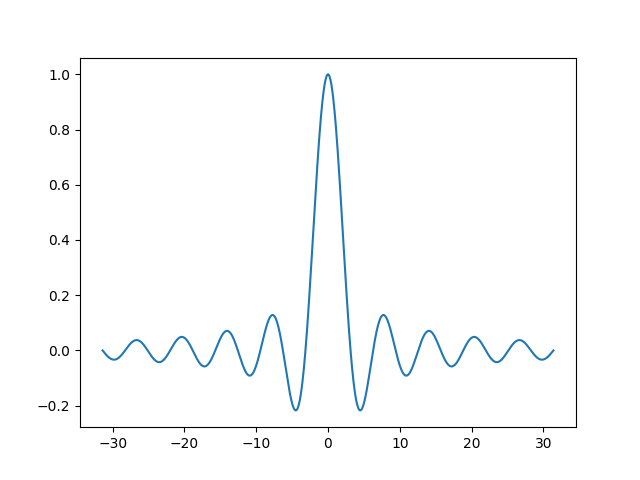
\includegraphics[width=.9\linewidth]{./graph.png}
\caption{\label{Test-figure}Test caption}
\end{figure}

Create an image by using [[./image$_{\text{file}}$ and close with two
brackets. Use C-c C-x C-v to view the image inline
% Emacs 24.5.1 (Org mode 8.2.10)
\end{document}
